\documentclass{article}

\usepackage{natbib}
\usepackage{graphicx}

\title{Machine Learning for Theorem Proving}
\author{Dobrik Georgiev, dgg30}


\begin{document}

\maketitle
\section{Introduction}

Machine Learning (ML) has found its application in many areas (natural language
processing, computer vision, etc) and it has succeeded in solving challenging
tasks where classical deterministic approaches have performed poorly. ML was
also successfully integrated into theorem proving, both interactive and
automatic. 

This survey focuses some of the ML techniques that have been applied for
theorem proving. It is organised in three main parts:
In section \ref{sec:background} I give a bit of background on theorem proving
(both automated and interactive). In section \ref{sec:ITP} the focus falls on
how ML is used in Interactive Theorem Proving and premise selection in
particular. Section \ref{sec:ATP} will investigate how ML can be used to guide
Automated Theorem Provers to improve their performance. Section
\ref{sec:conclusion} summarises the survey.

% \nocite{LearningToProveITP}

\section{Background}\label{sec:background}

Automated Theorem Provers (ATP) usually work by trying to prove a conjecture
using techniques similar to an algorithm. Many approaches exist -- resolution
with unification, tableaux, DPLL \citep{DPLL}, etc. Since these approaches can
take exponential time to check a formula, various heuristic (even some ML ones)
have been developed. Such provers, however, have been unable to make use of
high-level abstractions and reasoning that humans usually do, when developing
a complex proof or theory.

Proving complicated theories in higher-order logic in a `one click' manner has
turned out difficult to achieve and automate. Thus, a human factor has been
integrated in the process of theorem proving and Interactive Theorem Provers
(ITP) emerged \citep{HistoryITP}. In interactive theorem proving, users specify
high-level definitions and proofs using a sequence of so-called
\textit{tactics}\footnote{In an analogy to classic programming, these can be
viewed as the instructions.}. Low level details are then translated to ATP
formalisms and handed to an automated theorem prover, such as
E \citep{Eprover}, VAMPIRE \citep{VAMPIRE} or similar. As programming
languages, ITPs also have ``libraries'' (called \emph{theories} or \emph{theory
sets}), which contain various proofs, which can be imported and reused.

\section{Interactive Theorem Proving -- Machine \\ Learning for Premise Selection}\label{sec:ITP}

One of the problems when handling the proof of a conjecture to a lower-level
ATP arises when there are a lot of premises and facts (called \emph{axioms} in
theorem proving terminology), but very few of them are actually used in the
proof of the conjecture. Consequently, the ATP may attempt to use the
irrelevant facts which can in turn slow down the proving process or even lead
to a timeout\footnote{As proving a conjecture can be NP-complete in some
logics, most ATPs are run only for a fixed amount of time.}. This occurs
especially when a user is using a large theory or a set of several theories.
Ideally, we would want to pick \emph{only} those facts that are most relevant
to what we want to prove/necessary to the proof. This section presents how this
was approached using ML.

Some of the first experiments were preformed when translating
Mizar\footnote{Mizar is an assistant which mechanically checks proofs written
by humans. See \cite{MizarOverview} for an overview.} Mathematical Library,
which consisted of many formalised mathematical theories, to first-order logic
\citep{MizarProofAdvisor}. In an attempt to automatically select useful axioms
when proving theorems the Mizar Proof Advisor (MPA) was created. In the
implementation of MPA the symbols used in a proof of a theorem $T$ were used as
features and those were associated with the relevant proofs and facts used for
proving $T$. A naive Bayes was used for evaluating whether an axiom would be
useful for proving $T$. 

Building on the Mizar Proof Advisor, MaLARea \citep{MaLARea} was created using
the same idea as in \cite{MizarProofAdvisor} that features of a conjecture can
be associated with proofs which were successfully used when these features are
present. The goal of MaLARea is again to give a ranking of the axioms according
to their usefulness. What distinguishes this system from the above, is that it
implements \emph{deduce, learn from it, and loop} policy \citep[p.~3]{MaLARea}.
The policy's main loop consists of attempting to prove a set of problems (using
an ATP) with no more than a fixed number of axioms which were selected by
a Bayes classifier and under a fixed time limit. If nothing new is proven, the
axiom and time limits are increased. Upon a successful proof, they are reset to
their minimal values again and the proof is `learned'. It was shown that with
learning a `relevance filter', the number of problems that can be solved with
an ATP has increased drastically (cf. \S 3 of \cite{MaLARea}) compared to
passing all premises to the ATP.

The policy outlined above has been reused in the future as well, signifying the
contribution of \cite{MaLARea}. Some of the examples follow:
\begin{itemize}
    \item \textbf{MaLARea SG} \cite{MaLAReaSG} -- The system itself was
        improved with semantic guidance (cf. \cite{SRASS} for further details
        on semantic guidance).
    \item \textbf{MaSh} \cite{MaSh} employed it for improving Isabelle's
        Sledgehammer, which is a tool used for ATP proving of subgoals of
        a theory in Isabelle. Similar loop policy is used \citep[p.3]{MaSh} as
        well as the same algorithm -- still a naive Bayes, but a custom
        implementation, in order to improve performance (previous works used
        the off-the-shelf tool SNoW \citep{SNoW}).  A key difference to the
        previous work lie in how features of premises/proofs are created --
        instead of using simply the symbols, the nontrivial first-order
        patterns up to a given depth are used \citep[p.6]{MaSh}.
    \item \textbf{Learning with Flyspeck } -- the policy was also applied to
        the Flyspeck project \citep{FlyspeckProject}. One of the key differences
        here are that \cite{Flyspeck} claim that translation to ATP formalisms
        are sound in contrast to previous translations, e.g. Isabelle or Mizar
        to ATP, where one symbol from the corresponding ITP may be translated
        in several different ways. The motivation for a consistent translation
        is that external (heuristical) premise selection tools cannot be used
        otherwise and in their ranking scheme \cite{Flyspeck} use them as
        a `preprocessing' step of the (re)learning loop. Features used here are
        a variation of symbol preprocessing \citep[\S 4.1]{Flyspeck}, similar
        to what \cite{MaLARea} have.
\end{itemize}

Research time has also been devoted to improving the ML methodology for
premise selection, since this is a key component of good performance,
regardless whether we employ the aforementioned policy or not. Two of the
methods that have been tested are:
\begin{itemize}
    \item \textbf{Kernel Methods} -- \cite{PremiseSelection} used a premise
        selection algorithm based on kernel methods. The benefit is that such
        classifier can learn non-linear dependencies (it was proved in the
        paper that NB can learn only linear ones). 
    \item \textbf{k Nearest Neighbours (k-NNs)} -- \cite{FlyspeckFeatW} also
        showed that k-NNs with Inverse Document Frequency weighting of the
        features can give better results than naive Bayes. 
\end{itemize}

More recently, with the increasing popularity of Deep Learning, neural network
models have been applied to premise selection \citep{DeepMath}. The approach
taken embeds a pair of (conjecture, axiom) into a feature vector, which is then
processed by a neural network, resulting in a metric of how useful this axiom
would be. The training loss for a conjecture is defined as the worst ranking of
a premise which is known to be a true dependency (i.e. we know we cannot prove
the conjecture without it). Many neural network models were tested, inspired
both from Computer Vision and from Natural Language Processing. Results showed
that the models can give better results than the baseline of k-NN with
handcrafted features and in addition can be ``complementary'', i.e. even better
results are obtained when the neural network and hand engineered approaches are
combined -- 80\% of the problems used for testing were solved. \cite{DeepMath}
were the first to apply Deep Learning to theorem proving for premise selection
and presented how a variety of neural network models can be used for premise
selection.

The need for larger datasets was also identified. One such dataset is HolStep
\citep{HolStep}, featuring 2M statements (axioms/proofs/etc.) and 10K
conjectures making applying data hungry techniques like DL for premise
selection much easier. Other tasks together with baseline models \citep[\S 3,
4]{HolStep} were also proposed. This dataset was used in training other models,
e.g. the one from \cite{DeepGraph}.


Currently, the state-of-the-art uses ML/DL approaches for premise selection
(e.g. \cite{DeepGraph}). DL has also found use in generating full ITP
tactics and the focus in the last year or so is more on end-to-end Interactive
Theorem Proving proof generation, rather than only premise selection -- see
\cite{LearningToProveITP, GamePad, GNNsForTP} for example.

\section{Guiding ATPs}\label{sec:ATP}

As we saw in the last section, the approach of premise selection gives
a generic interface in which any ATP can be substituted and a variety of ML/DL
approaches can be employed. Despite its success, this approach has the drawback
that it uses the ATP as a black box -- it does not utilise the knowledge of
successful proofs to guide the ATP itself. In this section I give a summary of
some of the work done in using ML to guide an Automated Theorem Prover.

\begin{figure}[t]
    \centering
    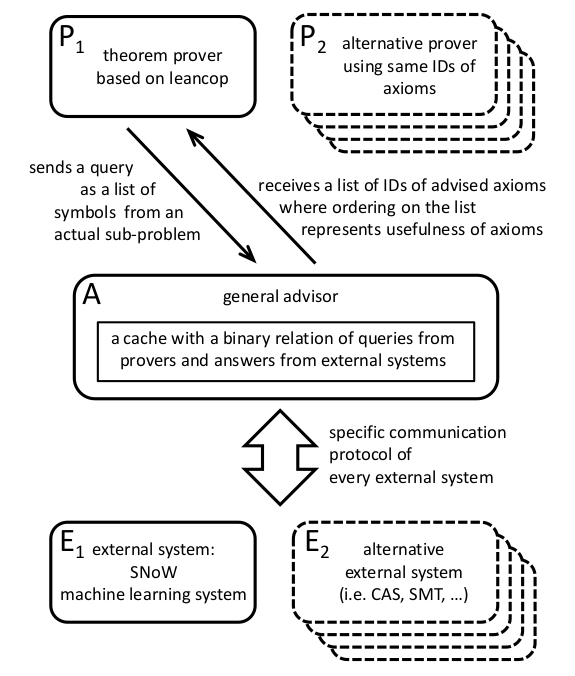
\includegraphics[width=0.5\textwidth]{malecop_arch.png}
    \caption{General architecture proposed by \cite{malecop}. Source: \cite{malecop}}
    \label{fig:malecop}
\end{figure}

\cite{malecop} proposed an `advisor' architecture to serve queries produced by
the ATP and created a Machine Learning Connection Prover (MaLeCoP) which used
ML to advise on the most useful clause for every extension step in a tableau
proof. The advisor system is depicted in Figure \ref{fig:malecop} -- \textbf{P}
represents a prover, \textbf{A} the advisor system, \textbf{E} the external
system. It can be noted that the idea of \emph{usefulness of axioms} is very
similar to what MaLARea does, but here, the actual proof state is also taken
into account and the advice is on what axioms are most useful for the next
steps, rather than for the \emph{whole} proof.

By substituting leanCoP \citep{leancop}, a connection tableaux prover for
\textbf{P}, SNoW \citep{SNoW} for \textbf{E} and a hand-implemented script for
\textbf{A}, MaLeCoP was born. Evaluation showed that MaLeCoP can produce
shorter by almost an order of magnitude proofs than those produced without
using any ML but there was a very high overhead due to recomputing the features
for similar states and the use of and communication to external ML system which
made the system impractical.

Based on the ideas of the above prototype, the system was greatly improved
\citep{femalecop}, making it both much faster than the prototype and better in
generalisation (90 unseen problems were proved compared to 7). Some of the
differences to MaLeCoP are:
\begin{itemize}
    \item efficient (re)computation of the features and relevance
        computation -- the feature vector of the proof state (as well as
        relevance scores) is updated incrementally on a tableau extension.
        % Although the features may be sometimes inaccurate due to substitutions
        % happening on a tableau extension this gives a significant speedup compared to
        % the previous prototype
    \item additional improvements on preprocessing the data and feature
        extraction, e.g. hash tables for faster accesses of the sum of
        occurences for a given features and more
    \item fast custom implementation of the ML advising system and its
        integration directly in the leanCoP code
        % to remove any communication
        % overhead
\end{itemize}
According to \cite{femalecop} and to the best of my knowledge, this was
the first time ML was (successfully) used for internally guiding an ATP.

\nocite{SatallaxProver}

The promising results of \cite{femalecop} inspired other works too and it was
applied to other ATPs as well, such as Satallax \citep{Satallax}. However it
was not until the work of \cite{Enigma} that ML was used for guiding an
\emph{state-of-the-art} ATP. This was achieved via efficient feature extraction
(term walks of length 3 \citep[\S 3.2]{Enigma}) and then utilising a large-scale
linear classifier. \cite{Enigma} again guided on the premise selection on every
ATP step, and reused the concept of the feedback loop from MaLARea
\citep{MaLARea}.

Reinforcement Learning algorithms have also been utilised. \cite{RLTP} showed that
it is possible to apply policy and value learning algorithms to guide
leanCoP. Although features were extracted in the same
hand-engineered way as \cite{Enigma}, results were very promising -- 40\% more
proofs were obtained, compared to the original prover.

The tediousness of engineering feature extraction and the success of applying
Deep Learning to premise selection \citep{DeepMath} inspired \cite{DNGPS} to
apply Deep Learning based guidance on an ATP. The E clause based prover was
chosen for the experiments. The DL guidance consists of taking an unprocessed
clause and the negated conjecture, embedding them and calculating the
probability that the clause would be used for proving the conjecture. Since
calculating the score for all clauses on every step was too expensive and pure
DL-based score was not practical hybrid approaches were proposed \citep[\S
5.2.1]{DNGPS}, which would initially use DL guidance but then would switch to
the ATP heuristics, when resources start running out. T

Given the success of the last two papers, current research mainly focuses on
using RL and DL \citep{GuidingTPbyRNNs,TowardsLonger}, but the exact
approach taken can vary between the papers, depending on the particular problem
identified and its solution.

\section{Conclusion}\label{sec:conclusion}

This assignment surveyed the two main applications of ML to theorem proving --
premise selection (usually associated with interactive theorem provers) and
internal guidance of automated theorem provers in the presence of large
theories. In both cases, that machine learning has been was used for filtering
the number of `step possibilities' (either the premises to use in ITP or the
next proof step in ATP). It was observed that the applied algorithms/techniques
are advantageous and can even lead to proofs which were impossible to prove
before with using heuristics for guiding the ATP.

Due to the emerge of more advanced techniques, such as deep learning, and to
the inherent difficulty of feature engineering, research has moved to using
neural networks to learn the embeddings of the conjectures/premises and how
these correlate. Despite that neural networks can be more computationally
expensive, when utilised correctly they could give even better results.

% \cite{FuchsGenetic} -- heuristic learned to be chosen with Gen Algo

% \cite{DomKnThmProv} -- inference control heuristics for equational deduction.
% Data from prev proofs, select equations that are likely to be used in new
% situations. 1st eval fn works by symbolic retrieval of generalized patterns
% from a kkn base, 2nd eval fn compiles the knowledge into abstract term
% evaluation trees. \textbf{Analyzed proof protocols} by representing knowledge
% about protocols'n'proofs 

% \cite{HighPerfATPAI} -- case-based reasoning, similarity concept, cooperation
% concept, reactive planning; still `learn' from previous successful proof
% attempts'

% \cite{FeatureBasedThmP} -- Learn search-guiding heuristics by employing
% features in a simple, yet effective manner. Features used to adapts a heuristic
% to a solved problem. Utilize heuristic profitably for related target problems.
% \textbf{Prediction of usefulness of a fact.} 

% SNoW \cite{SNoW} -- learning program that can be used as a general purpose
% mulit-class classifier and is specifically tailored for large number of
% features. Sparse Network of Winnows (not a typo). Sparse network of sparse
% linear functions over a pre-defined or incrementally acquired feature space.
% Several update rules may be used -- sparse variations of the Winnow update
% rule, the Perceptron or Naive Bayes. Multi class learner. Decisions either
% binary or continuous (confidence in [0, 1]).

% Proof General \cite{ProofGeneral} -- tool for developing proofs with ITP.
% Interaction based around proof script (seq of commands sent to ITP). Provides
% UI.

% Mizar proof advisor \cite{MizarProofAdvisor} -- MPTP (Mizar Problems for
% Theorem Proving) is system described; translates MML into ATPs and for
% generating thm proving problems corresponding to Mizar Mathematical Library.
% Mizar proof advisor used for selecting suitable axioms from the large library
% for an arbirtrary problem. Feature based ML framework, symbols are the features
% that characterise formulas. They had 40k targets and about 7k features.
% \textbf{SNoW} learning architecture used mainly (NLP archit, designed for large
% num of feat and targets).

% MizarMode \cite{MizarMode} -- Emacs authoring environment. Code-generating
% Code-Browsing Code-searching methods. Auto gen proof skeletons, semantic
% browsing of articles, structured viewing, proof advice using \textbf{machinee
% learning tools} like Mizar Proof Advisor. 

% Lightweight relevance filtering ... \cite{LightweightPaulson} -- relevance
% filtering methods, based on counting fn symbols in clauses. Signature based
% relevance filter. Not exactly ML?...

% The use of Data-Mining... \cite{DataMiningAFT} -- evaluate the applicability of
% data-mining techniques for tactics from large corpuses of proofs. Data mine
% information to find occuring patterns. Patterns are then evolved into tactics.
% Variable Length Markov Models used to predict next proof step.

% MaLARea \cite{MaLARea} -- simple metasystem iteratively combining deductive
% Automated Reasoning tools (now the E and the SPASS ATP systems) with a machine
% learning component (now the SNoW system used in the  naive  Bayesian  learning
% mode). Intended use -- large theories, i.e. large num of problems which in
% a consistent fashion use many axioms, lemmas, thms, etc. The system works in
% cycles of thm proving followed by ML from successful proofs, using the learned
% information to prune the set of available axioms for the next cycle. MPTP
% challenge - 142/252. Learning could be stated as creating an assoc of some
% features of the conjecture with proving methods. Features -- just symbols
% appearing in them. "Proving method" -- ordering of all av axioms. Goal -- given
% symbols, produces ordering of axioms, according to expected relevancy wrt the
% set of symbols. Sufficiently simple to implement and quite efficient in the
% first experiments with thm proving over Mizar library. Deduce, learn, loop
% implemented via growing axiom set and growing timelimit policy. First try to
% solve cheaply (min num axioms / most relevant, lowest timelimit). On success,
% learning performed on the newly available solution and axiom/time limit dropped
% to min values. No success -- increase limits. Details in paper. MLMLMLMLML SNoW
% used in NB mode, bcs of speed. One training example contains all the symbols of
% a solved conjecture w/ names of axioms needed. A bayes network is trained.
% Easier to just relearn every time. Trained classifier is used to prune the
% axiom set for the next runs -- we take all the unsolved conjectures and create
% a testing example from each by taking all its symbols. The classifier run on
% this printing (ordered) axioms. This is then used to select req num of axioms.
% Usage of previous results exists.

% SRASS \cite{SRASS} -- selection determined by semantics of the axioms and
% conjecture, heuristically ordered by a syntactic relevance measure. Many
% problems more solved. At each iter the process looks for a model of selected
% axioms and the neg of the conjecture. If no model found, then the conjecture is
% consequence. Otherwise, then an unselected axiom that is false in the model is
% moved to the set of selected axioms. Newly selected axiom excludes the model
% from the models of the selected axioms and neg conj, eventually leading to
% a situation where there are no models of the selected axioms and the negated
% conjecture. Unselected axioms selected in decreasing order of usefuleness.
% Syntactic relevance score for usefulness. Direct relevance is ratio of how many
% predicates and/or functors the have in common to how many they have overall.
% Contextual direct relevance uses `contextual intersection'.

% MaLARea SG \cite{MaLAReaSG} -- combines model-based and learning based methods
% for automated reasoning in large theories. The implementation is based on
% MaLARea. Extended by taking into account semantic relevance of axioms, similar
% to SRASS. Combined system outperforms both. Three extensions to selection of
% axioms. 1. check for countersatisfiability in runs where this is probable.
% Allows for countersatisfiability precheck to detect more cases when more axioms
% need to be added. 2. Use models found when a problem is found to be
% countersatisfiable, as an additional criterion for computing axiom relevance.
% Need to efficiently evaluate formulae in the models. 3. Extend axiom
% specification using a logical criterion: the set of axioms should exclude as
% many known models of the negated conjecture as possible. \textbf{Weird
% combination. Review!}

% MaLeCoP \cite{malecop} -- TABLEAU CALCULUS YAY!!! While in MaLARea
% learning-based axiom selection is done outside unmodified theorem provers, in
% MaLeCoP the learning-based selection is done inside the prover, and the
% interaction between learning of knowledge and its application can be much
% finer. The general design that we propose is as follows (see also Figure 1):
% The theorem prover (P) should have a sufficiently fast communication channel to
% a general advisor (A) that accepts queries (proof state descriptions) and
% training data (characterization of the proof state together with solutions
% and failures) from the prover, processes them, and replies to the prover
% (advising, e.g., which clauses to choose). The advisor A also talks to external
% system(s) (E). A translates the queries and information produced by P to the
% formalism used by a particular E, and translates E’s guidance back to the
% formalism used by P. At suitable time, A also hands over the (suitably
% transformed) training data to E, so that E can update its knowledge of the
% world on which its advice is based. A is free to spawn/query as many
% instances/versions of Es as necessary, and A is responsible for managing the
% guidance provided by them. Particular instances of Es that we have in mind are
% learning systems, however we believe that the tableau setting is also suitable
% for linking of SMT solvers, computer algebra systems, and all kinds of other AI
% systems, probably in a more straightforward way than for the resolution-based
% systems. SNoW again...

% Premise selection .. and kernel methods \cite{PremiseSelection} -- This  work
% develops  learning-based  premise  selection  in  two  ways.  First,a  newly
% available  minimal dependency  analysis  of  existing  high-level  formal
% mathematical proofs is used to build a large knowledge base of proof
% dependencies,  providing  precise  data  for  ATP-based  re-verification  and
% for  training premise selection algorithms.  Second, a new machine learning
% algorithm for premise selection based on kernel methods is proposed and
% implemented (Section 4 gives details) 0/1 features if sth appears in
% conjecture. Looking for a classifier fn which, given a conjecture c, estimates
% how useful p is for proving c. (still the aproach with chosing the best some
% premises) Maths explained nicely.

% Flyspeck \cite{Flyspeck} -- Trained on Flyspeck proofs. (HOL Light is an ITP)
% The procedure implemented for HOLLight is currently a combination of the
% external, internal, learning, and non-learning premise selection approaches.
% This procedure assumes the common ITP situations of a large library of (also
% definitional) theorems $T_i$ and their proofs $P_i$ (for definitions the proof
% is empty). The proofs refer to other theorems giving rise to a partial ordering
% of thms etended into their total chrono order. Procedure:
% \begin{enumerate}
%     \item characterisations of thms and proofs are extracted in a simple format
%     \item dependency data are obtained by running ATPs on the ATP problems created from the hollight deps, i.e. tms are re-proved. Preferred (it is smaller) data. Exported as 1
%     \item external premise selectors preprocess the thm characterizations and the proof deps. Multiple characterizations and proof dependencies may be used
%     \item when an new conjecture is stated in hollight its characterization is extracted and sent to the pretrained first stage premise selectors.
%     \item the first stage premise selectors work as rankers. For a given conjecture characterization they produce a ranking of the available theorems (premises) according to their (assumed) relevance for the conjecture.
%     \item The best ranked premises are used inside hollight to produce atp problems. Several thresholds on num of included premises are used, resulting in multiple versions of the ATP problems.
%     \item The ATPs are called on the problems. Some of the best ATPs run in a strategy-scheduling mode combining multiple strategies. Some of the strategies always use the SInE (i.e. local, second stage) premise selection (with different parameters) and some other strategies may to use SINE when the ATP problem is sufficiently large.
% \end{enumerate}
% \textbf{ML of Premise Selection}\\
% All the currently used first-stage premise selectors are machine learning
% algorithms trained in various ways on previous proofs. A number of machine
% learning algorithms can be experimented with today, and in particular
% kernel-based methods and ensemble methods have recently shown quite good
% performance on smaller datasets such as MPTP2078. Scaling hard on large corpus.
% So far this work uses mostly sparse implementation of a multiclass NB
% classifier (SNoW again...). Several other fast incremental learning algorithms
% were briefly tried -- perceptron and winnow algos (SNoW) and custom k-NN. Only
% k-NN produced enough additional prediction power. 

% At a given point during the library development, the training data available to
% the machine learners are the proofs of the previously proved theorems in the
% library. A frequently used approach to training premise selection is to
% characterize each proof $P_i$ of theorem $T_i$ as a (multi)set of theorems
% \{$T_{i_1}, ... T_{i_m}|T_{i_j} used in P_i$\} The training example will
% consist of the input characterization (features) of $T_i$ (features) and the
% output characterization of $T_i$ (labels) will be the multi set \{$T_i$\} and
% the previous set. Such training examples can be tuned in various ways. For
% example the output theorems may be further recursively expanded with their own
% dependencies,the input features could be expanded with the features of their
% definitions, various weighting schemes and similarity clusterings can be tried,
% etc. This is also mostly left to future general research in premise-selection
% learning. Once the machine learner is trained on a particular development state
% of the library, it is tested on the next theorem T in the chronological order.
% The input features are extracted from T and given to the trained learner which
% then answers with a ranking of the available theorems. This ranking is given to
% HOL Light, which uses it to produce ATP problems for T with varied numbers of
% the best-ranked premise
% (FOR THE PREVIOUS)
% custom implementation of the k-nearest neighbor (k-NN) machine-learning method,
% which computes for a new example (conjecture) the k nearest (in a given feature
% distance) previous examples and ranks premises by their frequency in these
% examples. (\\END)

% Stronger automation for Flyspeck... \cite{FlyspeckFeatW} -- 2 complementary AI
% methods used to improve strength of ai/atp service. First, several schemes for
% frequency-based feature weighting are explored in combination with
% distance-weighted k-nearest-neighbor classifier. A smaller improvement is
% obtained by evolving targeted E prover strategies on two particular premise
% selections, using the Blind Strategymaker (BliStr) system.  The  simplest  way  how  to  measure  the  similarity  of
% formulas  to  the  new  conjecture  is  to compute the overlap of their
% (sparse) feature vectors. Neglected  by  our  first  implementation  is
% however  the  sensitivity  of k-NN  to  feature  frequencies. Inverse Document
% Fequency weighting. 

% MaSh \cite{MaSh} -- Sledgehammer had relevance filter (syntactic similarity).
% Mash learns from succsessful proofs. Integrates easily. \emph{Draws on recent
% research in the context of Mizar and HOL Light.} CUSTOM version of a weighted
% sparse naiveB algo, that is faster than the NB in SNoW. Maintains persistent
% state and supports incremental, nonmonotonic updates.  The main technical
% difficulty is to perform the learning in a fast and robust way without
% interfering with other activities of the proof assistant. Power users can
% enhance the learning by letting external provers run for hours on libraries,
% searching for simpler proofs. A particularly strong filter, MeSh, is obtained
% by combining MePo (MEPO is paulsons thingie which selects based on num of
% relevant symbols) and MaSh. Implementations refines this in several ways --
% chained facts take absolutie priority, local facts are preferred to gloobal,
% first order facts preferred to hol ones; rare symbols are weighted more
% heavily; etc. Mepo tents to perform best on that contain some rare symbols,
% otherwise it discriminates poorly. There is also issue of starvation: the
% filter with its iterative expansion of the set of relevant symbols effectively
% performs a best first search and may ignore some relevant facts close to the
% root. Provers given ranked selected facts. Time limit and number of facts vary
% (the classic setting). Once a proof is found, Sledgehammer miinimizes it by
% invoking the prover repeatedly with subsets of the facts it refers to. 
% \\\textbf{The ML engine}\\
% Default algorithm NB adapted to fact selection. Manipulates thm proving
% concepts in an abstract way. Handcrafted features. Sources of proofs -- all
% facts in theories. Most interesting lemmas, those written by man. (see paper
% for math details)

% MaLARea04 \cite{MaLARea04} -- seems like nothing new...

% FEMaLeCoP (great names btw) \cite{femalecop} -- FEMaLeCoP is a connection
% tableau theorem prover based on leanCoP which uses efficient implementation of
% internal learning-based guidance for extension steps. Despite the fact that
% exhaustive use of such internal guidance can incur a significant slowdown of
% the raw inferencing process, FEMaLeCoP trained on related proofs can prove many
% problems that cannot be solved by leanCoP. Femalecop is the first ai/atp system
% convincingly demonstrating that guiding the internal inference algorithms of
% theorem provers by knowledge learned from previous proofs can significantly
% improve the performance of the provers.  In the MaLeCoP(Machine Learning
% Connection Prover) experiment we have shown that in principle it is possible to
% significantly prune the internal search space of leanCoP. In this work, we
% devise much stronger learning-based guidance for connection tableau by
% developing an AI/ATP system where the learning-based guidance is an optimized
% and tightly integrated part of the core inferencing algorithm and data
% structures. The basis of FEMaLeCoP is the OCaml version of leanCoP. We advise
% the selection of clause for every tableau extension step. (see paper) We use
% a fast custom OCaml implementation of the naive Bayes algorithm that learns the
% association of the features of the proof states (see below) with the
% contrapositives that were used for the successful tableau extension steps in
% previous proofs. We characterize the proof state as a weighted vector of
% symbols and/or (possibly generalized) terms extracted from all the literals on
% the active path. (see details) An optional problem-specific data-filtering step
% is to use the k-nearest neighbor (k-NN) algorithm for further restriction of
% the relevant training data. If this is used, we first find the k solved
% problems whose conjectures are (in the feature metric) closest to the current
% conjecture, and extract the training examples only from such problems.
% (INTEGRATED LIKE AN INTERNAL SYSTEM)

% Mizar40 \cite{Mizar40} -- 40\% of thms solved in the MML. To achieve that,
% a large suite of AI/ATP methods is employed and further developed. We implement
% the most useful methods efficiently, to scale them to the 150000 formulas in
% MML. The main body of our work thusconsists of the following steps: (DETAILS IN
% PAPER...).  Nothing really interesting or 'grand'

% A learning based fact selector... \cite{LearnBasedFactSelIsabel} -- MaSh
% reintroduction...

% DeepMath \cite{DeepMath} --  "We propose a two stage approach for this task
% that yields good results for the premise selection task on the Mizar corpus
% while avoiding the hand-engineered features of existing state-of-the-art
% models. To our knowledge, this is the first time deep learning has been applied
% to theorem proving on a large scale." 4 main contributions: 1) demonstration
% for the first time that neural network models are useful for aiding in large
% scale automated logical reasoning without the need for hand-engineered features
% 2) Comparison of various network architectures 3) A method of semantic-aware
% “definition”-embeddings for function symbols that improves the generalization
% of formulas with symbols occurring infrequently 4) Analysis showing that neural
% network based premise selection methods are complementary to those with
% hand-engineered features. Motivation from NLP (see paper)\\
% OverviewOfApproach\\
% Pairwise relevance -- predicting the probability that a given axiom is useful
% for proving a given conjecture. The conjecture and axiom sequences are
% separately embedded into fixed length real vectors, then concatenated and
% passed to a third network with 2 fully connected layers and logistic loss.
% During training time, the two embedding networks and the joined predictor path
% are trained jointly. As discussed in section 3, we train our models on premise
% selection data generated by a combination of various methods, including
% k-nearest-neighbor search on hand-engineered similarity metrics. We start with
% a first stage of character-level models, and then build second and later stages
% of word-level models on top of the results of earlier stages.

% Character level models -- We begin by avoiding special purpose engineering by
% treating formulas on the character-level using an 80 dimensional one-hot
% encoding of the character sequence. These sequences are passed to a weight
% shared network for variable length input. (see paper)
% Word-level models -- The character-level models are limited to word and
% structure similarity within the axiom or conjecture being embedded.  However,
% many of the symbols occurring in a formula are defined by formulas earlier in
% the corpus, and we can use the axiom-embeddings of those symbols to improve
% model performance.

% HOLstep \cite{HolStep} -- In this paper, we introduce a new dataset based on
% Higher-Order Logic (HOL) proofs, for the purpose of developing new machine
% learning-based theorem-proving strategies. Reasons for hol given in paper and
% how dataset is extracted. Several possible tasks are outlined.

% End-to-End differentiable proving \cite{EndToEndDiffProving} -- doesn't fit in
% the picture (nice paper otherwise)

% Reinforcement Learning of Theorem Proving \cite{RLTP} -- Thm proving algo that
% uses practically no domain heuristics for guiding its connection-style proof
% search. Instead, it runs many Monte-Carlo simulations guided by reinforcement
% learning from previous proof attempts. We produce several versions of the
% prover, parameterized by different learning and guiding algorithms. In this work, we remove this requirement, since it basically means that all shorter proof candidates have to be tried before a longer proof is found.

% \textbf{bare prover} Our bare prover is based on a previous reimplementation
% [23] of leanCoP in OCaml (mlCoP).Unlike the Prolog version,mlCoP uses an
% explicit stack for storing the full proof state (used for the ML part).  We
% first modify mlCoP by removing iterative deepening, i.e., the traversal
% strategy that makes sure that shorter (shallower) tableaux are  tested  before
% deeper  ones.   Instead,  the  bare  prover  randomly  chooses  extension  and
% reduction steps operating on the current goal, possibly going into arbitrary
% depth. Next, we add playouts and search node visit counts. A play out of length
% d is simply a sequence of d consecutive extension/reduction steps (inferences)
% from a given proof state(a tableau with a selected goal). Inferences  thus
% correspond  to actions and  are  similar  to  moves  in  games.   We  represent
% inferences as integers that encode the selected clause together with the
% literal that connected to the goal.  Instead of running one potentially
% infinite playout, the bare prover can be instructed to play n playouts of
% length d. Each playout updates the counts for the search nodes that it visits.
% Search nodes are encoded as sequences of inferences starting at the empty
% tableau. A playout can also run without length restrictions until it visits
% a previously unexplored search node. The  next  modification  to  this  simple
% setup  are bigsteps done  after b playouts.   They  correspond to moves that
% are chosen in games after many playouts.  Similarly, instead of starting all
% playouts always from scratch (empty tableau) as above, we choose after the
% first b playouts a particular single inference  (bigstep),  resulting  in
% a  new bigstep  tableau.   The  next b playouts  will  start  with  this
% tableau, followed by another bigstep, etc.

% \textbf{rlcop} extends the bare prover with (i) Monte-Carlo tree search balancing exploration and exploitation using the UCT formula. To implement Monte-Carlo tree search, we maintain at each search node i the number of its visits $n_i$, the total reward $w_i$, and its prior probability $p_i$. This is the transition probability of the action (inference) that leads from i's parent node to i. If no policy learning is used, the prior probabilities are all equal to one. The total reward for a node is computed as a sum of the rewards of all nodes below that node. In the basic setting, the reward for a leaf node is 1 if the sequence of inference s results in a closed tableau, i.e., a proof of the conjecture. Otherwise it is 0. (actually is slightly different -- see paper)

% Great paper, but need to review some RL for presentation.

% \textbf{GENERATING TACTICS}

% \cite{LearningToProveITP}
% \cite{SEPIA}
% \cite{TacticToe}
% \cite{LearningToProveTactics}
% \cite{GamePad}
% \cite{HOList}
% \cite{Bridge2014}

% \textbf{OTHER}
% \cite{GNNsForTP}


\bibliographystyle{apalike}
\bibliography{refs.bib}

\end{document}
